\chapter{Methods}

This chapter introduces the outline of this project, the datasets used in the experiments, the hardware and software information, the detailed 
explanation of the experiment design and the construction of deep learning models.

\section{Projects Outline}
The project was performed in following steps:
\begin{itemize}
    \item Access and preprocess the datasets if necessary.
    \item Apply rCOMMIT experiment on the target datasets
    \item Extract pseudo ground truth from the experiment results.
    \item Construct deep learning models.
    \item Train and tune the models to achieve stable performance.
    \item Compare the results between models.
    \item Compare the results with previous research.
  \end{itemize}

\section{Datasets}
In this project, the preprocessed datasets of six different subjects from the young adult data set of the Human Connectome Project \cite{vanessenWUMinnHumanConnectome2013} are used as raw data.
The tractograms are generated by the authors of \cite{TractSegFastAccurate} with iFOD2 \cite{tournierImprovedProbabilisticStreamlinesa} and MRtrix3 \cite{tournierMRtrix3FastFlexible2019}. 
Ten million streamlines are generated for each subject and the length of streamlines are restricted to be in the range between 40 mm to 250 mm.
The tracking was further constrained by anatomical priors based on the segmentation of different tissue types in the brain \cite{smithAnatomicallyconstrainedTractographyImproved2012}.
And the ten million streamlines cover the whole white matter of each subject. 

In the Fig \ref{fig:hist}, it shows the distribution of streamline length, the number of sampling points and the relationship between them.
From the figures, the number of streamlines decreases when the length gets longer. The length of the streamline and the number of sampling points 
are highly correlated. The streamlines here in tck files are loaded and summarized with the Python library Dipy \cite{garyfallidisDipyLibraryAnalysis2014}.

\begin{figure}[ht]
    \centering
    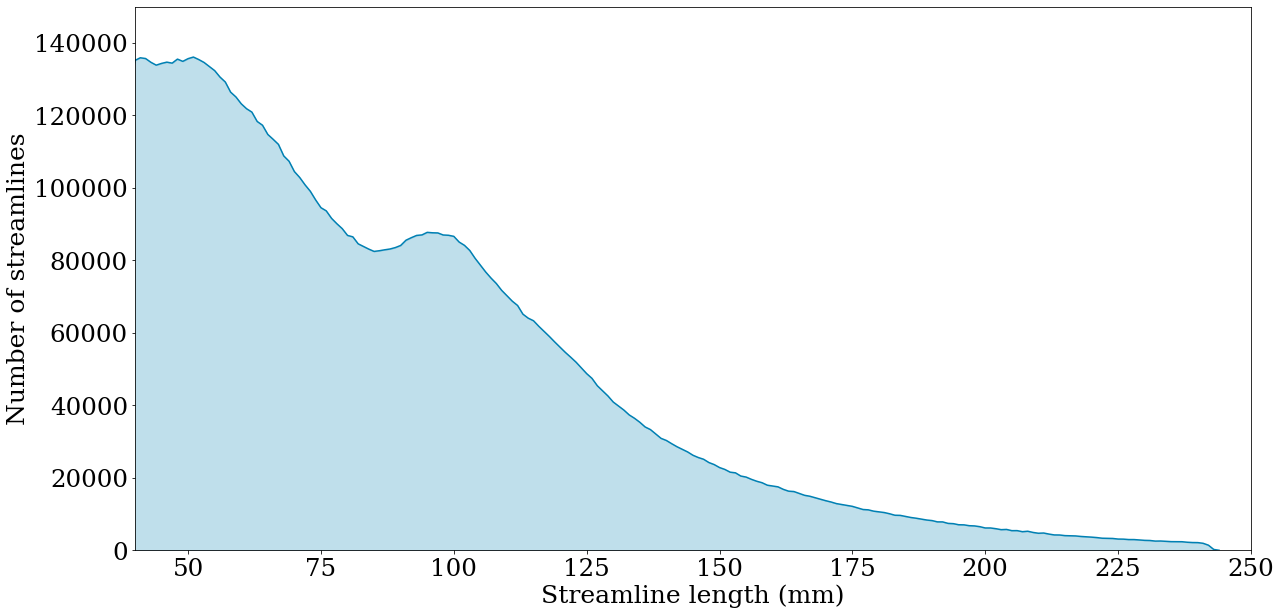
\includegraphics[width= 13cm]{figures/distribution.png}
    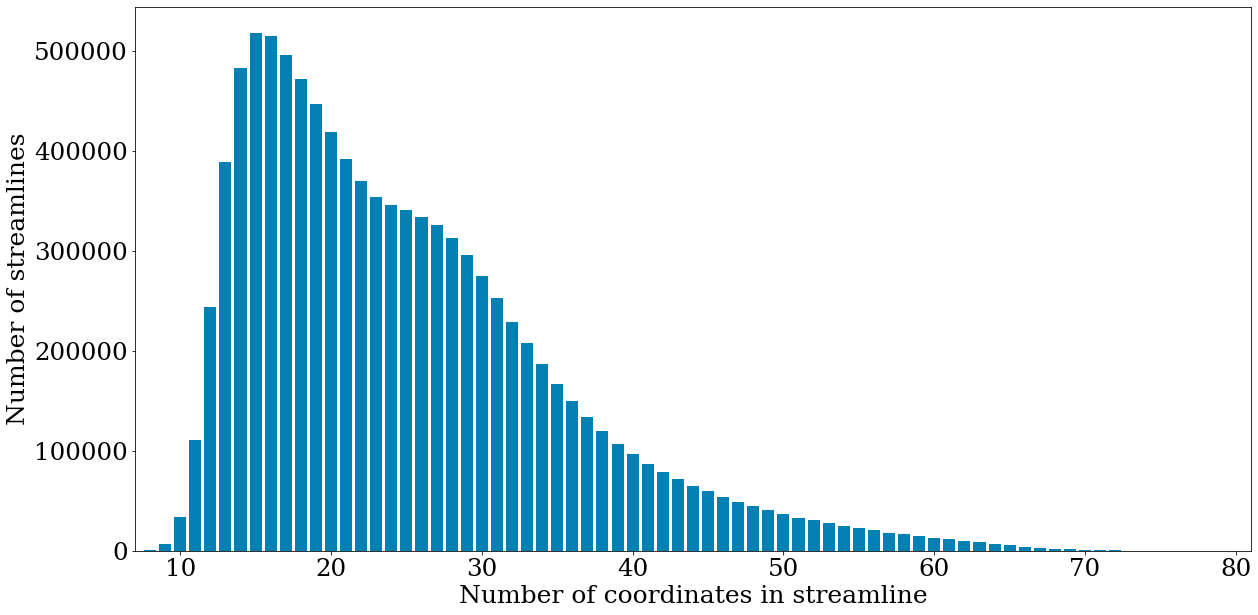
\includegraphics[width= 13cm]{figures/histogram.png}
    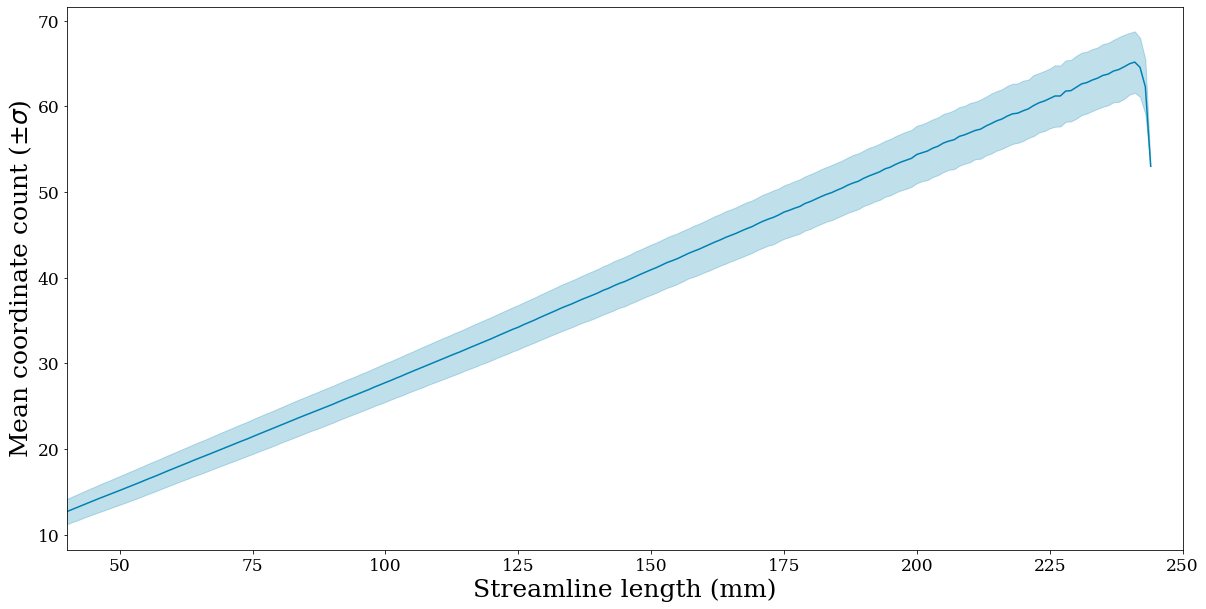
\includegraphics[width= 13cm]{figures/length_points.png}
    \caption{An overview of the input dataset from one subject. Distribution of the number of points and length of streamlines of ten million streamlines. 
    Top: histogram of the number of points per streamline. 
    Middle: histogram of streamline length in mm. 
    Bottom: correlation plot between streamline length and the mean number of sampling points with standard deviation (light blue).}
    \label{fig:hist}
\end{figure}

\section{Hardware and Software}
Two Nvidia GPUs are used for the training of deep learning models in this project, which respectively are of 4 GB and 11 GB memory. 
The latter GPU is deployed on a platform, Medical Artificial Intelligence Aggregator (MAIA) \cite{MAIA}, which aims to integrate and promote collaborations in the medical field.

COMMIT \cite{daducciCOMMITConvexOptimization2015} is used as the main filtering tool in the experiments. 
SIFT \cite{smithSIFTSphericaldeconvolutionInformed2013} is used in the previous research from which the results are compared in this study.
MRtrix3 \cite{tournierMRtrix3FastFlexible2019} helps visualize the data to check the white matter region is covered by the streamlines. 
The type of raw data is originally in tck file, and a script from ScilPy realizes the conversion between tck and trk files.
Python library Dipy takes care of postprocessing and analysing the tractograms in the training with DL models.
The neural network is built based on TensorFlow, and the monitor of the training process is done with TensorBoard.

\section{Randomized COMMIT (rCOMMIT)}
Finding anatomical ground truth for tractogram has always been a challenge, and there is no ground truth for the filtering method.
In addition, the results from the existing filtering methods are not consistent. Both problems make the filtering methods less plausible.
To Avoid biases and extract plausible information from the filtering methods, randomized COMMIT is purposed. 
The main idea of this method is to use multiple assessments from COMMIT on the same streamline in different subsets in order to classify streamlines into different groups.
The filtering process can be regarded as a binary classification, since in one time running of COMMIT, the streamline is either accepted or rejected by the filtering method.
The results from multiple times of filtering are seen as votes that are either positive or negative.

Another concern is the bias of the size of the dataset. Usually for a tractogram of 10 million streamlines, around 2\% - 2.5\% streamlines are remained after filtering.
During the filtering, when the remaining streamlines are too small to guarantee the stability of the computation, the filtering method would terminate the process.
To investigate the performance of COMMIT in different sizes, 
multiple subsets are generated from the raw data. From the raw dateset to the smallest dateset, the size of subsets is automatically chosen, by halving
the subset size. And the smallest size is set to be 2.5\% of the input size. Therefore, all the used sizes include $SS= \left \{  1\times 10^7, 5\times 10^6, 2.5\times 10^6, 1.25\times 10^6, 6.25\times 10^5, 5\times 10^5, 2.5\times 10^5 \right \}$ 

Fig \ref{fig:pipe} shows the whole pipeline of rCOMMIT and the pseudo algorithm of the pipeline is shown in \ref{fig:algo}. 
The process of rCOMMIT will be explained more in details with the pseudo algorithm. rCOMMIT will run on all subsets with predefined
size $n \in SS$, and for each $n$ the repetition time $k$ is calculated according to the formula below:
\begin{gather}\label{computek}  
    k = \tau M/n
\end{gather}
$M$ is the original number of streamlines in the tractogram, and $\tau$ is the parameter set in the experiments, 
which indicates the purposed average filtering times by COMMIT for the streamlines. This parameter helps achieve enough votes for classifying streamlines into groups.
For example, with $\tau=5$, the repetition time $k \in \left \{5, 10, 20, 40, 80, 100, 200 \right \}$ for each size in $SS$.
Therefore, with multiple times of filtering, the acceptance rate (AR) of each streamline can be obtained, which is computed below:
\begin{gather}\label{AR}
    AR(s) = \frac{P(s)}{P(s)+ N(s)}
\end{gather}
$AR(s)$ refers to the acceptance rate for the streamline $s$ after receiving all the votes from the experiment in different sizes.
$P(s)$ stands for the positive votes while $N(s)$ are the negative votes.
It's worthy mentioning that each subset is randomly sampled from the raw data. 
Although a target average number of filtering is set, but the number of occurrences of each streamline in the subsets is not ensured, 
which means the numbers of votes for the streamlines can be various.

\begin{figure}[ht]
    \centering
    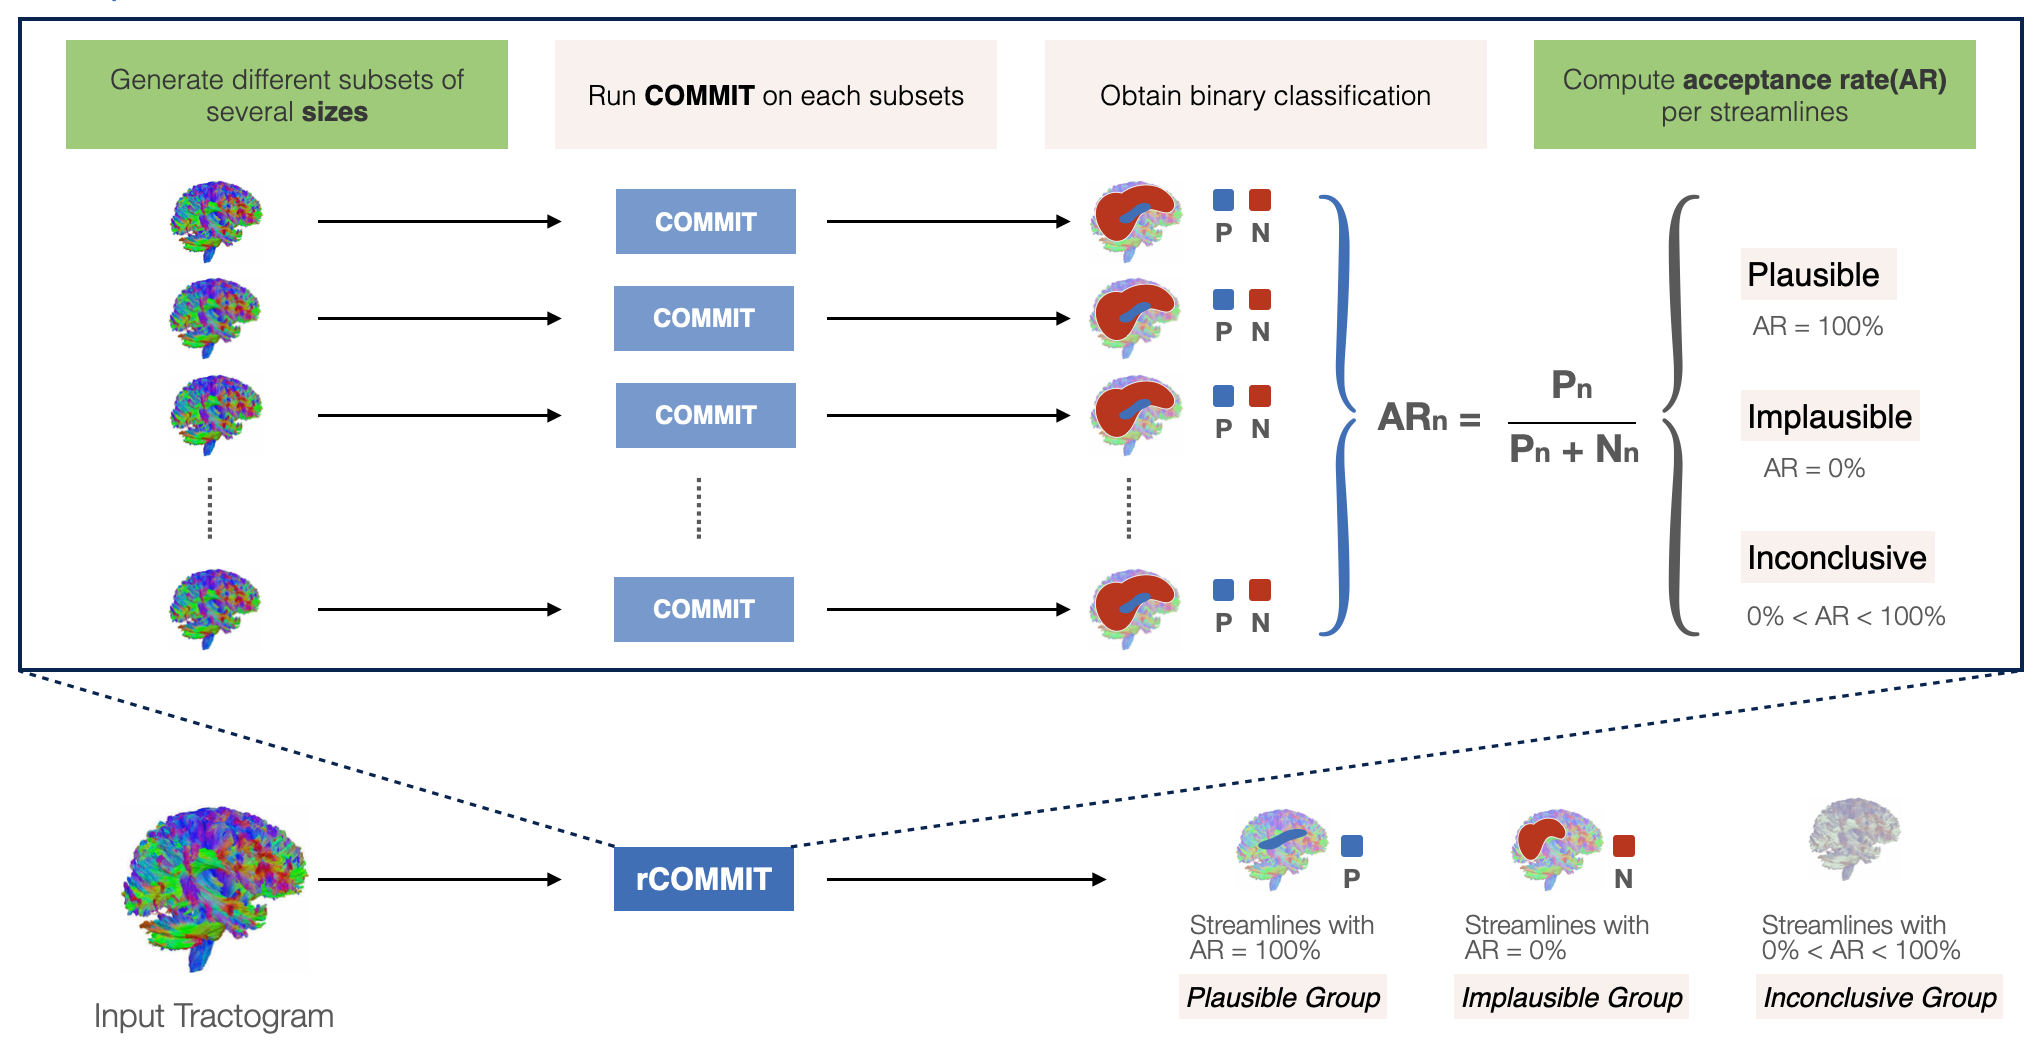
\includegraphics[width= 16cm]{figures/pipe.jpg}
        \caption{The pipeline of rCOMMIT. 
        }
    \label{fig:pipe}
\end{figure}


\begin{algorithm}
    \caption{Pseudocode of rCOMMIT. For the chosen subset size $n$, $k$ random subsets of the tractogram are randomly extracted and filtered with COMMIT to 
    receive the index of the accepted and rejected streamlines $subset_i^P$ and $subset_i^N$. These are used to update the number of votes and compute the acceptance rate in the end.}
    
    \KwIn{
    \begin{tabular}{ll}
    $T = \{t_1, t_2, \ldots, t_{M}\}$ : tractogram,\\
    $SS = \{s_1, s_2, \ldots, s_N\}$ : subset sizes
    \end{tabular}}
    
    \KwOut{
    \begin{tabular}{ll}
    $P = \{p_1, p_2, \ldots, p_M\}$: accepted times,\\
    $N = \{n_1, n_2, \ldots, n_M\}$: rejected times
    \end{tabular}}
    
    \BlankLine
    \BlankLine
    %\Begin{
    Initialize $P$ and $N$ with zeros\\
    \ForAll{$n \in SS$}{
    Initialize $P_n$ and $N_n$ with zeros\\
    $k \gets \tau M/n$\\
    \For{$i \in \{1, \ldots, k\}$}{ 
    $subset_i \gets \{r_1, \ldots,r_n\} \subseteq T$, where $ r_{1, \ldots, n}$ are randomly selected from $T$\\
    $[subset_{i}^P, subset_{i}^N] \gets COMMIT(subset_i)$\\
    $P_n(subset_i^P) \gets P_n(subset_i^P)+1$\\
    $N_n(subset_i^N) \gets N_n(subset_i^N)+1$
    }
    $P= P+P_n$\\
    $N= N+N_n$\\
    
    }
    \label{fig:algo}
    
\end{algorithm}

\section{Pseudo Ground Truth}

After receiving all the votes from the experiments, the acceptance rate can be obtained for almost every streamline.
The pseudo ground truth is based on the acceptance rate of each streamline. This step is based on the very important assumption in this study.
The streamline with higher acceptance rate indicates its better ability to survive from filtering. These streamline are more plausible than those with lower acceptance rate.
To better classify streamlines, strict conditions are made to separate them into three groups:

\begin{enumerate}
    \item Plausible group when $AR = 100\%$
    \item Implausible group when $AR = 0\%$
    \item Inconclusive group when $0\% <AR< 100\%$
  \end{enumerate}

Streamlines being in the plausible group means that they are always accepted by the COMMIT, while in the implausible group the streamlines are always rejected.
These two groups can also be labeled as true and false. Those in the inconclusive group receives inconsistent votes from the COMMIT. 

\section{Deep Learning Streamline Classifier}
rCOMMIT is purposed to extract plausible information from the filtering methods. To further investigate the different properties between groups and the potential
of deep learning methods in filtering field, neural networks classifiers are built and trained on the labeled dataset from the last step.
In the experiment, the classifiers are trained for the binary classifications among three classes and the multi-class tasks.

\subsection{Data Preprocessing}
To make the datasets from different subjects more appropriate for the training process, preprocessing steps are conducted.
Originally, each streamline consists of multiple sampling points and each point has three coordinates. 
First, the streamline coordinates are normalized to the range of -1 and 1 in each dimension using the maximum and minimum values per subject.
However, the sampled points for each streamline are various. Secondly, to standardize the input of each streamline, they are resampled to the same 
number of points. A big number of points from the input streamline might cause expensive computation, while too few points might contain 
inadequate information. So the medium number of streamline points among the training subjects is chosen to be the resampled number, which is 23.
Linear interpolation is used to realize this step. Last, the shape of the streamlines is changed from 3-D into 1-D by flattening the vector. 
The original coordinates are 
In beginning of the preprocessing steps, all the tck files of tractograms are loaded as Numpy arrays, 
so the preprocessing steps can be easily operated with Numpy. 

\subsection{Model Construction}

For the classification tasks, the Convolutional Neural Network (CNN) is widely used. In our study, the classifiers are built on the CNN architecture.
Each classifier contains two 1-D conventional layers with ReLU activation function and the kernel sizes 5 and 3. 
A max-pooling layer with pool size 2 is applied after each of them. Then conventional layers are then followed by the dense layer with a dropout chance.
Last, the dense layer is connected with either one or multiple neurons as output, depending on the classification tasks.

\begin{figure}[ht]
    \centering
    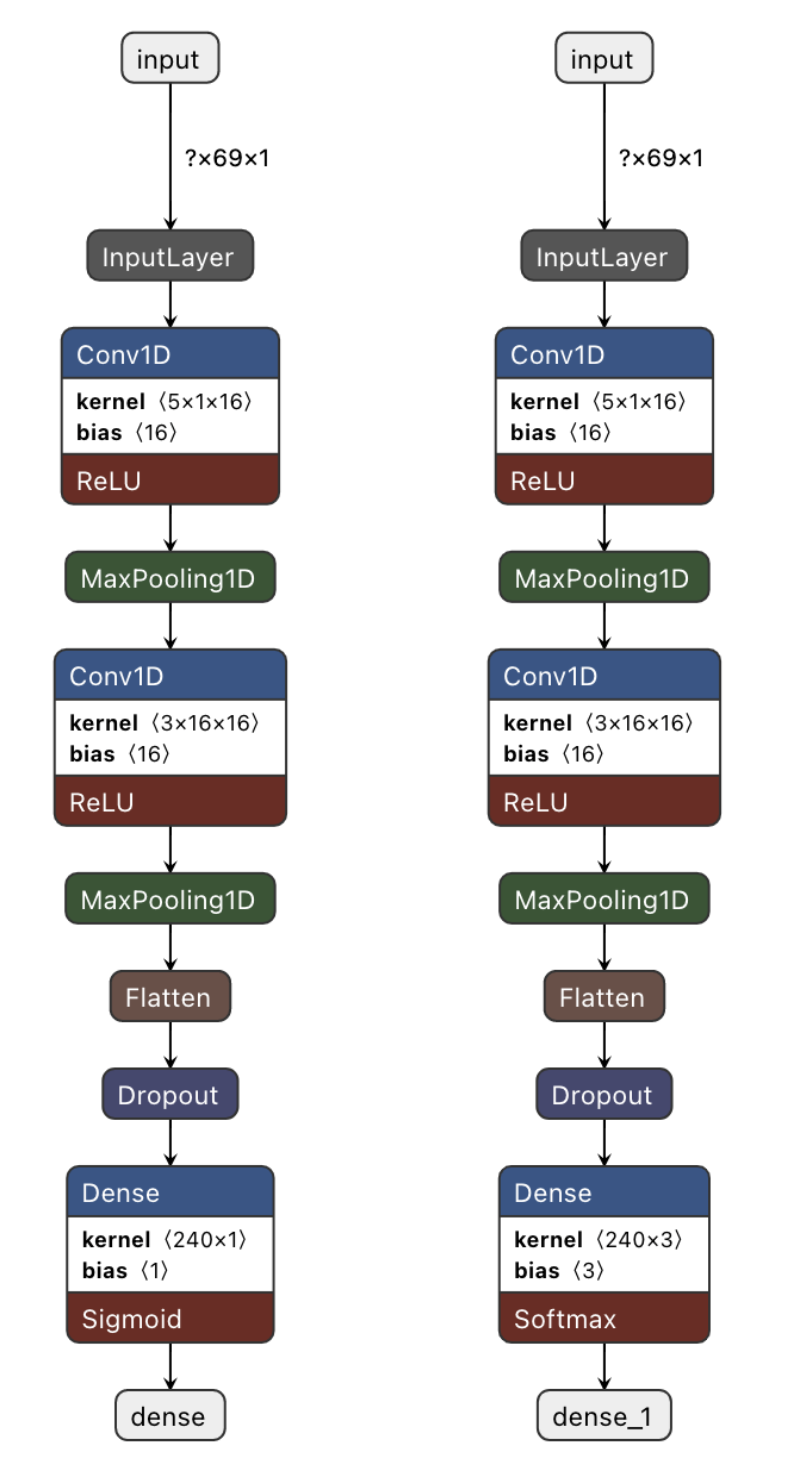
\includegraphics[width= 10cm]{figures/models.png}
        \caption{Architecture of the classifiers. Left: binary classifier. Right: multi-class classifier. 
        The only difference is in the last dense layer. The binary classifier uses one neuron with sigmoid activation, 
        while the multi-class classifier uses multiple output neurons with softmax activation. In our case, the output neurons are 3 for the multi-class classifier.}
    \label{fig:models}
\end{figure}

To do: about RNN model

\subsection{Balance Data Generator}

The data generator is designed to solve the imbalance problem of the dataset. In a binary classification, 
when there is a big imbalance between two classes, for example one class over 90\% and the other one less than 10\%,
the classifier is prone to predict the result to be the bigger class on the normal batch of input. 

In our study, the dataset is mainly based on the filtering method which rejects the majority of the streamlines. 
The disproportion in the dataset is expected. Thus, the data generator is used to over-sample the smaller class for the training and testing.
The batch size is defined to be 60, so it is flexible with two classes and three classes of the input data. 
The epoch size is defined by the larger class and each sub-batch from this class will be seen at least once.
While the sub-batch from the smaller class will be reused and shuffled when it is exhausted during an epoch.









